\documentclass[12pt]{article}
\usepackage{amsmath}
\usepackage{tikz}
\usepackage{float}
\begin{document}
\title{Electrical Engineering 102, Homework 4}
\date{November 1st, 2018}
\author{Michael Wu\\UID: 404751542}
\maketitle

\section*{Problem 1}

\paragraph{a)}

\begin{enumerate}
    \item Since the left term has a period of \(\frac{2}{3}\) and the right term has a period of \(\frac{1}{2}\), we know that \(f(t)\) has a period of \(2\).
    So we need to calculate the Fourier series coefficients \(c_k\) to obtain a solution in the form of
    \[f(t)=\sum_{k=-\infty}^\infty c_k e^{jk\pi t}\]
    which is given by
    \[c_k=\frac{1}{2}\int_0^2 f(t)e^{-jk\pi t}\,dt\]
    Rewriting \(f(t)\) in complex form yields
    \[f(t)=\frac{1}{2}\left(e^{j3\pi t}+e^{-j3\pi t}\right) + \frac{1}{4j}\left(e^{j4\pi t}-e^{-j4\pi t}\right)\]
    and so
    \[c_k=\frac{1}{2}\int_0^2 \frac{1}{2}\left(e^{j(3-k)\pi t}+e^{-j(3+k)\pi t}\right) + \frac{1}{4j}\left(e^{j(4-k)\pi t}-e^{-j(4+k)\pi t}\right)\,dt\]
    We see that \(c_k=0\) for all \(k\neq -4,-3,3,4\). We obtain the following coefficients.
    \begin{align*}
        c_{-4}&=-\frac{1}{4j}\\
        c_{-3}&=\frac{1}{2}\\
        c_3&=\frac{1}{2}\\
        c_4&=\frac{1}{4j}
    \end{align*}
    Therefore we have the Fourier series
    \[f(t)=-\frac{1}{4j}e^{-j4\pi t}+\frac{1}{2}e^{-j3\pi t}+\frac{1}{2}e^{j3\pi t}+\frac{1}{4j}e^{j4\pi t}\]
    which is the same as the complex form written above.
    \item The period is 1 so we have a Fourier series of the form
    \[f(t)=\sum_{k=-\infty}^\infty c_k e^{jk2\pi t}\]
    where the Fourier series coefficients are given by
    \begin{align*}
        c_k &= \int_0^1 e^{-2t} e^{-jk2\pi t}\, dt\\
        &= \int_0^1 e^{-(2+jk2\pi)t}\, dt\\
        &=-\frac{e^{-(2+jk2\pi)}-1}{2+jk2\pi}\\
        &=-\frac{e^{-2}-1}{2+jk2\pi}
    \end{align*}
    \item The period is 3 so we have a Fourier series of the form
    \[f(t)=\sum_{k=-\infty}^\infty c_k e^{jk\frac{2\pi}{3} t}\]
    where the Fourier series coefficients are given by
    \begin{align*}
        c_k&=\frac{1}{3}\left(\int_0^1 2e^{-jk\frac{2\pi}{3} t}\, dt + \int_1^2 e^{-jk\frac{2\pi}{3} t}\, dt\right)\\
        &=\frac{1}{3}\left(-\frac{2(e^{-jk\frac{2\pi}{3}}-1)}{jk\frac{2\pi}{3}} -\frac{e^{-jk\frac{4\pi}{3}}-e^{-jk\frac{2\pi}{3}}}{jk\frac{2\pi}{3}}\right)\\
        &=\frac{1-e^{-jk\frac{2\pi}{3}}}{jk\pi}+\frac{e^{-jk\frac{2\pi}{3}}-e^{-jk\frac{4\pi}{3}}}{jk2\pi}
    \end{align*}
\end{enumerate}

\paragraph{b)}

\begin{enumerate}
    \item The function \(z(t)\) will have a period of \(T=T_1\) and have a Fourier series of the form
    \[z(t)=\sum_{k=-\infty}^\infty Z_k e^{jk\frac{2\pi}{T} t}\]
    Because the exponential terms are the exact same as in the Fourier series of \(x(t)\) and \(y(t)\), the coefficients for \(z(t)\) are given by \(Z_k=X_k+Y_k\).
    \item The function \(w(t)\) will have a period of \(T=T_1=2T_2\) and have a Fourier series of the form
    \[w(t)=\sum_{k=-\infty}^\infty W_k e^{jk\frac{2 \pi}{T} t}=\sum_{k=-\infty}^\infty W_k e^{jk\frac{\pi}{T_2} t}\]
    The exponential at a given \(k\) corresponds to the same exponential in the Fourier series of \(x(t)\), while it corresponds to the exponential with index \(\frac{k}{2}\) in the Fourier
    series of \(y(t)\) if \(k\) is even. Thus we have
    \[W_k=
        \begin{cases}
            X_k & \text{if }k\text{ is odd}\\
            X_k+Y_{\frac{k}{2}} & \text{if }k\text{ is even}
        \end{cases}
    \]
\end{enumerate}

\section*{Problem 2}

\paragraph{a)}

The period of this signal is \(T_0\), and it has the Fourier series coefficients
\[g_k=
    \begin{cases}
        c_k+1 & k=0\\
        c_k & k\neq 0
    \end{cases}
\]

\paragraph{b)}

The period of this signal is \(T_0\), and it has the Fourier series coefficients \(g_k=c_{-k}\).

\paragraph{c)}

The period of this signal is \(T_0\), and it has the Fourier series coefficients \(g_k=c_ke^{-jk\omega_0 t_0}\).

\paragraph{d)}

The period of this signal is \(\frac{T_0}{a}\), and it has the Fourier series coefficients \(g_k=c_k\).

\section*{Problem 3}

\paragraph{a)}

We say that \(f(t)\) is an eigenfunction of an LTI system \(S\) if and only if \(y(t)=S(f(t))=af(t)\) where \(a\) is some constant. Given an impulse
response \(h(t)\) we have that
\[S(f(t)) = \int_{-\infty}^{\infty} h(\tau)f(t-\tau)\, d\tau\]
Thus we want to show that
\[af(t) = \int_{-\infty}^{\infty} h(\tau)f(t-\tau)\, d\tau\]
Given that \(f(t)=\cos(\omega_0 t)\), we can rewrite \(f(t)\) in its Fourier series form which is \(f(t)=\frac{1}{2}e^{j\omega_0 t} + \frac{1}{2}e^{-j\omega_0 t}\),
which allows us to plug into this formula and evaluate the following.
\begin{align*}
    a\left(\frac{1}{2}e^{j\omega_0 t} + \frac{1}{2}e^{-j\omega_0 t}\right)
    &=\int_{-\infty}^{\infty} h(\tau)\frac{1}{2}e^{j\omega_0 (t-\tau)} + \frac{1}{2}e^{-j\omega_0 (t-\tau)}\, d\tau\\
    &=\left(\int_{-\infty}^{\infty} h(\tau)e^{-j\omega_0\tau}\, d\tau\right)\frac{1}{2}e^{j\omega_0 t}\\
    &\qquad+\left(\int_{-\infty}^{\infty} h(\tau)e^{j\omega_0\tau}\, d\tau\right)\frac{1}{2}e^{-j\omega_0 t}\\
    &=b\frac{1}{2}e^{j\omega_0 t}+c\frac{1}{2}e^{-j\omega_0 t}
\end{align*}
In this case we have that \(b\) and \(c\) are constants because the integrals do not depend on \(t\). But assuming \(\omega_0 \neq 0\), the two integrals can differ and \(b\neq c\).
Therefore there may be no constant \(a=b=c\) that makes the above equation true. So \(\cos(\omega_0 t)\) is not an eigenfunction of all LTI systems.

\paragraph{b)}

Consider the LTI system \(S\) characterized by the impulse response
\[h(t)=
    \begin{cases}
        1 & 0\leq t \leq 1\\
        0 & \text{otherwise}
    \end{cases}
\]
If the function \(f(t)=t\) is an eigenfunction of this system \(S\), we would expect that \(at=S(f(t))=h(t)*t\). Evaluating the convolution integral we get the following.
\begin{align*}
    h(t)*t&=\int_0^1 t-\tau\, d\tau\\
    &=t-\frac{1}{2}
\end{align*}
Because of the \(\frac{1}{2}\) term, this cannot take the form of \(at\) which means that \(t\) is not an eigenfunction of \(S\). Therefore \(t\) is not an eigenfunction of all LTI systems.

\section*{Problem 4}

\paragraph{a)}

The output of the first multiplication will be \(f(t)=e^tx(t)\). Then the output of the LTI system is \(g(t)=S_1(f(t))=f(t)*h(t)\), given the impulse function \(h(t)\). Then
the output of the second multiplication will be \(y(t)=e^{-t}g(t)\). Using substitution this yields
\[y(t)=e^{-t}(f(t)*h(t))=[(e^tx(t))*h(t)]e^{-t}\].

\paragraph{b)}

Let \(h^\prime(t)=e^{-t}h(t)\). Then we can rewrite \(y(t)\) as follows.
\begin{align*}
    y(t)&=[(e^tx(t))*h(t)]e^{-t}\\
    &=e^{-t}\int_{-\infty}^\infty e^\tau x(\tau) h(t-\tau)\, d\tau\\
    &=\int_{-\infty}^\infty x(\tau) e^{-(t-\tau)} h(t-\tau)\, d\tau\\
    &=\int_{-\infty}^\infty x(\tau) h^\prime(t-\tau)\, d\tau\\
    &=\int_{-\infty}^\infty h^\prime(\tau) x(t-\tau)\, d\tau
\end{align*}

\paragraph{c)}

The previous result indicates that the system that maps \(x(t)\) to \(y(t)\) is defined by a convolution integral, namely \(h^\prime(t)*x(t)\). Convolution is by definition linear and
time invariant, so this is an LTI system. The impulse response of this system \(h_\text{eq}(t)\) can be found by evaluating \(h^\prime(t)*\delta(t)\), giving us
\[h_{eq}(t)=h^\prime(t)=e^{-t}h(t)\]

\paragraph{d)}

The impulse response is the derivative of the step response. This means that the impulse response is given by
\[h(t)=u(t-1)\]
So the system \(S_1\) is causal because the impulse response is zero when \(t<0\). The system \(S_1\) is not stable. An example that shows this is the step response, which is is a bounded
input that produces the ramp function, an unbounded output.

The overall equivalent system that maps \(x(t)\) to \(y(t)\) has the impulse response given by
\[h_\text{eq}(t)=e^{-t}u(t-1)\]
It is also causal since the impulse response is zero when \(t<0\).
We can check if it is stable by finding the bounds of \(y(t)\) given a bounded \(x(t)\). Let \(|x(t)|<B\) for all \(t\). Then we have
\begin{align*}
    \left|\int_{-\infty}^{\infty} h_\text{eq}(\tau)x(t-\tau)\, d\tau\right|&\leq B \left|\int_{-\infty}^{\infty} h_{eq}(\tau)\, d\tau\right|\\
    &=B\left|\int_1^\infty e^{-\tau}\, d\tau\right|\\
    &=\frac{B}{e}
\end{align*}
Therefore we have that given an input bounded by \(B\), we get an output bounded by \(\frac{B}{e}\). So the overall equivalent system is stable.

\section*{Problem 5}

\paragraph{a)}

I implemented the function using the following code.
\begin{verbatim}
function fn=problem5a(Dn,omega0,t)
    function ft=evalAtPoint(Dn, omega0, t)
    ft=0;
    N=(length(Dn)-1)/2;
    for n=-N:N
        ft=ft+Dn(n+N+1)*exp(1i*omega0*n*t);
    end
    end
fn=arrayfun(@(t)(evalAtPoint(Dn, omega0, t)), t);
end
\end{verbatim}

\paragraph{b)}

I graphed the plots using the following code.
\begin{verbatim}
index=-10:10;
c10=-(exp(-2)-1)./(2+2i.*index*pi);
index=-50:50;
c50=-(exp(-2)-1)./(2+2i.*index*pi);
index=-100:100;
c100=-(exp(-2)-1)./(2+2i.*index*pi);
t=-2:0.001:2;
f10=problem5a(c10,2*pi,t);
f50=problem5a(c50,2*pi,t);
f100=problem5a(c100,2*pi,t);
set(gcf,'color','w');
plot(t,f10);
xlabel('t');
ylabel('f_{10}(t)');
export_fig problem5b-10.pdf;
plot(t,f50);
xlabel('t');
ylabel('f_{50}(t)');
export_fig problem5b-50.pdf;
plot(t,f100);
xlabel('t');
ylabel('f_{100}(t)');
export_fig problem5b-100.pdf;
\end{verbatim}
The plots are shown below.
\begin{figure}[H]
    \begin{center}
        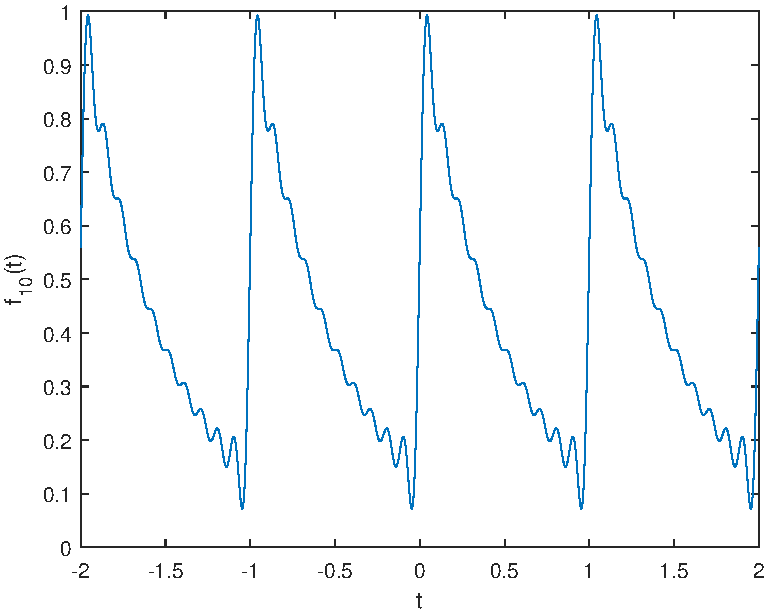
\includegraphics[width=2.5in]{problem5b-10.pdf}
        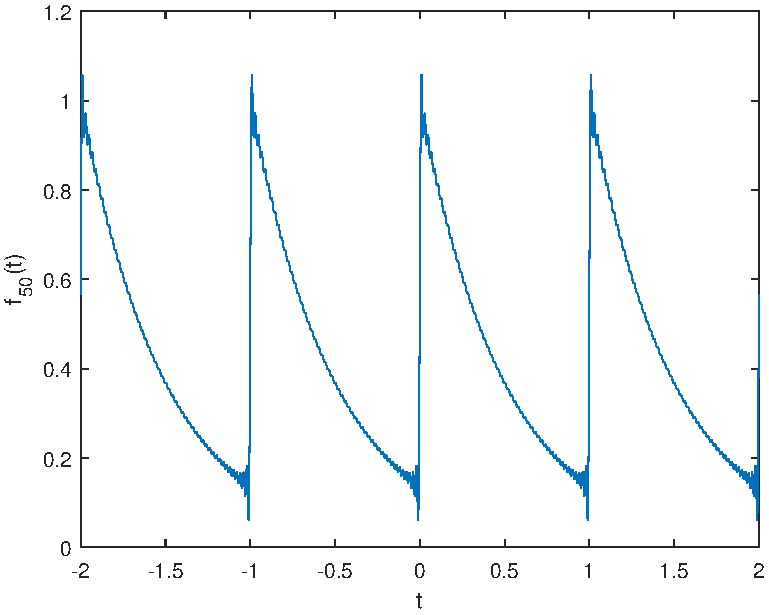
\includegraphics[width=2.5in]{problem5b-50.pdf}
        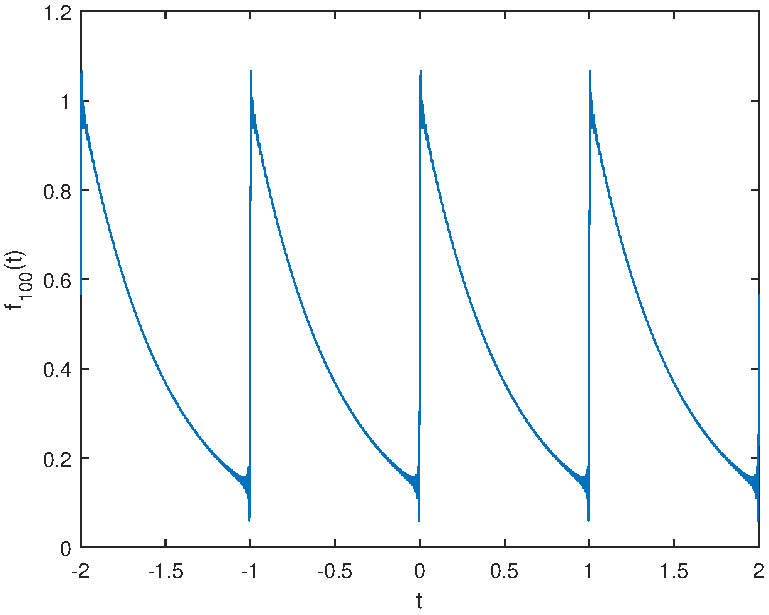
\includegraphics[width=2.5in]{problem5b-100.pdf}
    \end{center}
\end{figure}

\end{document}